\documentclass[xcolor=x11names,compress,usenames,dvipsnames,mathsans]{beamer}
\usepackage{textpos}
\usepackage[greek,english]{babel}
\usepackage{natbib}
\usepackage{wrapfig,color,dashrule,epsfig,graphicx}
\usepackage{pstool,psfrag}
\newcommand{\calt}{\color{red} } % alert color
\newcommand{\ccom}{\color{blue} } % commentary color

\newcommand{\redtext}[1]{\color{UOEred}{#1}\color{UOEblue}}

\newcommand{\link}[1]{\textbf{\textcolor{PMS3025}{\underline{#1}}}}
\definecolor{NewRed}{rgb}{0.8, 0.0, 0.0}


 %% Beamer Layout %%%%%%%%%%%%%%%%%%%%%%%%%%%%%%%%%%
\usetheme{Edinburgh}
\usecolortheme{edinburgh}
\usefonttheme[onlylarge]{structurebold}
\setbeamertemplate{itemize items}[circle]

\setbeamerfont{title}{size={\fontsize{13}{20}}}
\setbeamercolor*{palette tertiary}{fg=black,bg=black!10} 
\setbeamercolor*{palette quaternary}{fg=black,bg=black!10} 
\setbeamercolor{alerted text}{fg=red}
\setbeamercolor{sidebar}{bg=red!25!blue,fg=white}

\def\ci{\perp\!\!\!\perp} 

\setbeamercovered{transparent}

\addtobeamertemplate{footline}{}
{
  \begin{textblock*}{100mm}(.845\textwidth,-0.57cm) 
    
    
\includegraphics[height=0.5cm, width=1.8cm]{225px-Epcc_logo.jpg}
  \end{textblock*}
} 



\addtobeamertemplate{frametitle}{}
{
  \begin{textblock*}{100mm}(.935\textwidth,-0.645cm) 
	
\includegraphics[scale=.1]{crest_rb.eps}
  \end{textblock*}
}


\usepackage{graphicx} % Allows including images
\usepackage{booktabs} % Allows the use of \toprule, \midrule and \bottomrule in tables



%\setbeamercovered{transparent}

%----------------------------------------------------------------------------------------
%	STYLE STUFF -- section title slides
%----------------------------------------------------------------------------------------

\AtBeginSection[]{
  \begin{frame}
  \vfill
  \centering
  \begin{beamercolorbox}[sep=8pt,center,shadow=true,rounded=true]{title}
    \usebeamerfont{title}\insertsectionhead\par%
  \end{beamercolorbox}
  \vfill
  \end{frame}
}


%----------------------------------------------------------------------------------------
%	TITLE PAGE
%----------------------------------------------------------------------------------------

\title[Parallel-in-time methods with ML]{Parallel-in-time methods with ML} 
% The [Short Title] appears at the bottom of every slide, the {Full Title} is only on the title page

\author[author]{Viktor Csomor \\
\textit{s1984842@ed.ac.uk} \\
\vspace{1em}

\includegraphics[scale=.8]{logo_colour.pdf}
} % Your name

\date{\today}

\begin{document}

\begin{frame}
\titlepage % Print the title page as the first slide
\begin{center}
Supervisors:
Rupert Nash, Anna Roubíčková
\end{center}
\end{frame}

\begin{frame}
\frametitle{Overview} % Table of contents slide, comment this block out to remove it
\tableofcontents % Throughout your presentation, if you choose to use \section{} and \subsection{} commands, these will automatically be printed on this slide as an overview of your presentation
\end{frame}

%----------------------------------------------------------------------------------------
%	PRESENTATION SLIDES
%----------------------------------------------------------------------------------------

%------------------------------------------------
%\section{Section Title} % Sections can be created in order to organize your presentation into discrete blocks, all sections and subsections are automatically printed in the table of contents as an overview of the talk
%------------------------------------------------

\section{Motivation}

\begin{frame}
\frametitle{Differential equations}
\begin{itemize}
	\item numerous scientific and engineering problems are described by time-dependent differential equations
	\item ODEs and PDEs
	\item many different numerical methods exist for solving them \cite{suli2003}
\end{itemize}
\end{frame}

\begin{frame}
\frametitle{Parallelism}
\begin{itemize}
	\item traditionally, parallelised across the system or across space \cite{gear1988}
	\item good weak scaling, limited strong scaling
	\item but for some problems only wall time matters (e.g. stock trading)
	\item need to exploit parallelism better to reduce wall clock time
\end{itemize}
\end{frame}

\begin{frame}
\frametitle{Parallel-in-time methods}
\begin{itemize}
	\item solution parallelised across the time steps
	\item more CPU time, less wall clock time
	\item parareal algorithm \cite{parareal} for solving IVPs
	\item relies on two operators, coarse $G$ and fine $F$
	\item for every iteration, $G$ executed serially, $F$ in parallel
	\item $G$ must be fast but preferably also accurate enough
\end{itemize}
\end{frame}

\begin{frame}
\frametitle{Parareal algorithm}
\begin{figure}[!htb]
\begin{center}
\resizebox{1.0\hsize}{!}{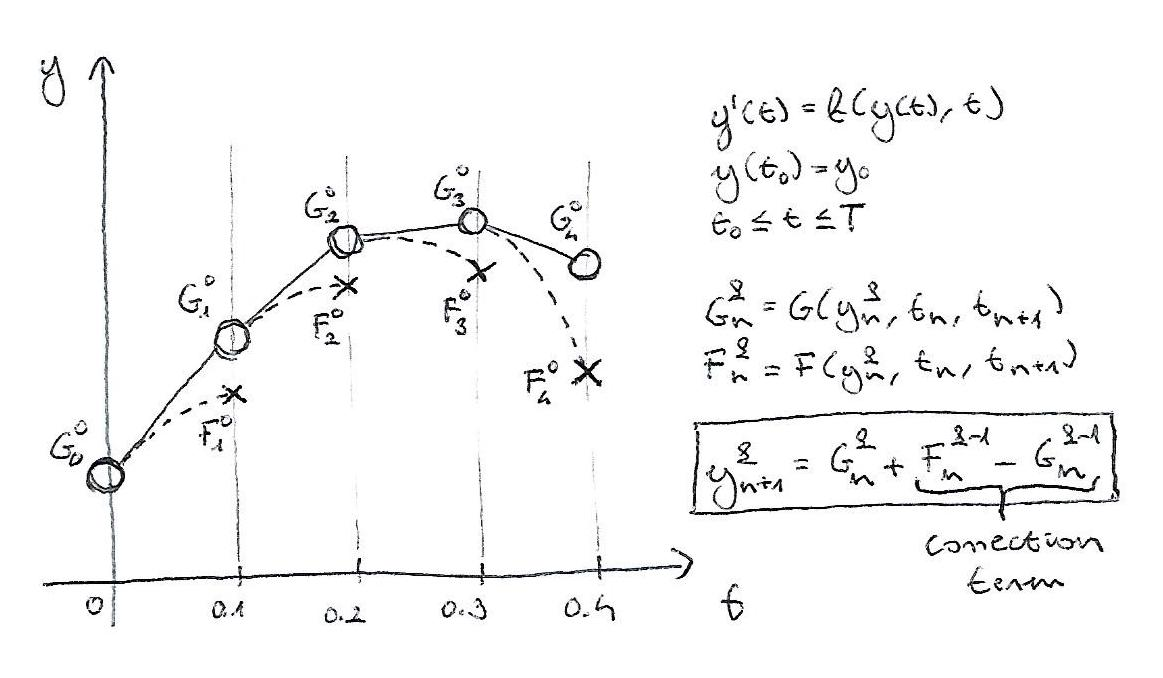
\includegraphics{parareal.jpg}}
\end{center}
\end{figure}
\end{frame}

%------------------------------------------------

\section{Hypotheses}

\begin{frame}
\frametitle{Hypotheses}
\begin{enumerate}
	\item an ML (regression) model can be trained and used as $G$ to solve differential equations in a parareal framework
	\item for some problems, the ML model based $G$ operator is better than traditional coarse operators in terms of performance and accuracy
	\item for some problems, the ML accelerated parareal framework achieves shorter wall time than a conventional parareal algorithm or a state-of-the-art traditional solver using the same number of CPU cores
	\begin{enumerate}[a]
	    \item training time ignored
	    \item training time taken into account
	\end{enumerate}
\end{enumerate}
\end{frame}

%------------------------------------------------

\section{Related work}

\begin{frame}
\frametitle{Related work}
\begin{itemize}
    \item neural network for solving time-dependent differential equations \cite{regazzoni2019}
    \item neural network to approximate the gradients of high-dimensional PDEs \cite{han2018}
    \item physics informed neural network (PINN) for solving PDEs \cite{raissi2017} \cite{sirignano2018} \cite{lu2019}
    \item parareal solver using a PINN as $F$ \cite{meng2019}
\end{itemize}
\end{frame}

%------------------------------------------------

\section{Challenges}

\begin{frame}
\frametitle{Challenges}
\begin{itemize}
    \item numerical analysis is a complex field
    \item fast moving area of research
    \item many potential avenues (PDE solving methods, model training, tech stack)
    \item aiming high
\end{itemize}
\end{frame}

%------------------------------------------------

\section{Plan}

\begin{frame}
\frametitle{Implementation}
\begin{itemize}
    \item develop a simple parareal framework
    \begin{itemize}
        \item[$-$] already implemented first version in C with POSIX threads 
    \end{itemize}
    \item construct an ML model (PINN vs standard models)
    \item train the model using targets provided either by $G$ or $F$
    \item automatise the model training as part of the framework
    \item use the trained model for inference as $G$
    \item extend the framework to discretise PDEs or handle PDEs directly through the model
\end{itemize}
\end{frame}

\begin{frame}
\frametitle{Problem iterations}
\begin{itemize}
    \item ODE (Lotka-Volterra)
    \item simple PDE (2D diffusion)
    \item high-dimensional PDE (Black-Scholes)
\end{itemize}
\end{frame}

\begin{frame}
\frametitle{Performance}
\begin{itemize}
    \item compare the ML version of $G$ to traditional ODE solvers of similar accuracy
    \item compare the performance of the parareal framework to traditional ODE and PDE solvers and analyse the impact of the model training on performance
    \item try different ML models (linear regression, ANN, RNN, etc.)
    \item take advantage of Cirrus' new GPUs
\end{itemize} 
\end{frame}

\begin{frame}
\frametitle{Tech stack}
\begin{itemize}
    \item C/C++ faster than Python but most scientific Python libraries are just wrappers on top of C bindings
    \item Python better suited for ML and numerical solver libraries are easier to use
    \item mpi4py \cite{dalcin2005} for distributed computing
    \item scikit-learn \cite{pedregosa2011} and keras \cite{chollet2015} for ML
    \item FEniCS \cite{fenics2015} (finite element) and FiPy \cite{fipy2009} (finite volume) to compare performance against
\end{itemize}
\end{frame}

%------------------------------------------------

\begin{frame}[allowframebreaks]
\frametitle{References}
\bibliographystyle{unsrt}
\bibliography{ref}
\end{frame}


\end{document} 